\documentclass{beamer}
%\documentclass[handout]{beamer}

\mode<presentation>
{% AnnArbor
%\usetheme{AnnArbor}
  %\usetheme{Boadilla}
  \usetheme{CambridgeUS}
 %\usetheme{Madrid}
  \setbeamercovered{transparent}
}

\usepackage{fontspec,xltxtra,xunicode,moreverb}

\usepackage[french]{babel}
% \usepackage{beamerthemesplit} // Activate for custom appearance

\usepackage{listings}
\usepackage{color}

\definecolor{mygreen}{rgb}{0,0.6,0}
\definecolor{mygray}{rgb}{0.5,0.5,0.5}
\definecolor{mymauve}{rgb}{0.58,0,0.82}

\lstset{ 
  backgroundcolor=\color{white},   % choose the background color; you must add \usepackage{color} or \usepackage{xcolor}; should come as last argument
  basicstyle=\footnotesize,        % the size of the fonts that are used for the code
  breakatwhitespace=false,         % sets if automatic breaks should only happen at whitespace
  breaklines=true,                 % sets automatic line breaking
  captionpos=b,                    % sets the caption-position to bottom
  commentstyle=\color{mygreen},    % comment style
  deletekeywords={...},            % if you want to delete keywords from the given language
  escapeinside={\%*}{*)},          % if you want to add LaTeX within your code
  extendedchars=true,              % lets you use non-ASCII characters; for 8-bits encodings only, does not work with UTF-8
  firstnumber=1000,                % start line enumeration with line 1000
  frame=single,	                   % adds a frame around the code
  keepspaces=true,                 % keeps spaces in text, useful for keeping indentation of code (possibly needs columns=flexible)
  keywordstyle=\color{blue},       % keyword style
  language=Python,                 % the language of the code
  morekeywords={*,...},            % if you want to add more keywords to the set
  numbers=left,                    % where to put the line-numbers; possible values are (none, left, right)
  numbersep=5pt,                   % how far the line-numbers are from the code
  numberstyle=\tiny\color{mygray}, % the style that is used for the line-numbers
  rulecolor=\color{black},         % if not set, the frame-color may be changed on line-breaks within not-black text (e.g. comments (green here))
  showspaces=false,                % show spaces everywhere adding particular underscores; it overrides 'showstringspaces'
  showstringspaces=false,          % underline spaces within strings only
  showtabs=false,                  % show tabs within strings adding particular underscores
  stepnumber=1,                    % the step between two line-numbers. If it's 1, each line will be numbered
  stringstyle=\color{mymauve},     % string literal style
  tabsize=2,	                   % sets default tabsize to 2 spaces
  % title=\lstname                   % show the filename of files included with \lstinputlisting; also try caption instead of title
}


%% No navigation symbol.
\setbeamertemplate{navigation symbols}{}
\beamertemplatenavigationsymbolsempty

%\setbeameroption{hide notes}

% \newcommand{\mypause}{\pause}
\newcommand{\mypause}{~}

\newcommand{\mypauseBeforeExercise}{\pause}

\newcommand{\elvrm}{\rm}
\newcommand{\fivrm}{\rm}
\newcommand{\sixrm}{\rm}
\newcommand{\sevrm}{\rm}
\newcommand{\egtrm}{\rm}
\newcommand{\ninrm}{\rm}
\newcommand{\tenrm}{\rm}
\newcommand{\twlrm}{\rm}
\newcommand{\frtnrm}{\rm}
\newcommand{\svtnrm}{\rm}
\newcommand{\twtyrm}{\rm}
\newcommand{\twfvrm}{\rm}

\newcommand{\ex}{{\bf Exemple}}
\newcommand{\afor}{\bf for}
\newcommand{\ato}{\bf to}
\newcommand{\ado}{\bf do}
\newcommand{\aendo}{\bf endo}
\newcommand{\esp}{\hspace{0.5cm}}

\newcommand{\sal}{\sum_i \mu_i}
\newcommand{\sbet}{\sum_j \nu_j}
\newcommand{\If}{\mbox{\bf if }}
\newcommand{\Then}{\,\mbox{\bf then }}
\newcommand{\titre}[1]{\title{{{\color{red} \large \bf #1}}}}

% Needed for course 2.
\newcommand{\Zn}{{\bf Z}^n}
\newcommand{\Z}{{\bf Z}}
\newcommand{\N}{{\bf N}}
\newcommand{\Np}{{\bf N}^p}

\newcommand{\alfa}{\textsc{alpha}}
\newcommand{\alfacase}{\mbox{\bf case}}
\newcommand{\alfaesac}{\mbox{\bf esac}}
\newcommand{\zset}{\mathbb{Z}}

\newcommand{\sys}{{\bf system}}
\newcommand{\real}{{\bf real}}
\newcommand{\of}{{\bf of}}
\newcommand{\lett}{{\bf let}}
\newcommand{\tel}{{\bf tel}}
\newcommand{\returns}{{\bf returns}}
\newcommand{\boolean}{{\bf boolean}}
\newcommand{\true}{{\bf true}}
\newcommand{\false}{{\bf false}}

\newcommand{\pomme}{\texttt{cmd}}
\newcommand{\alalign}{{$\hookleftarrow$}}

\newcommand{\pyth}{{\sc Python}}
\newcommand{\prog}[1]{\alert{\texttt{#1}}}

\title{Introduction à l'informatique, avec \pyth{}}
% \author{Patrice Quinton}
\author{Lilian Besson}
\date{2020--2021\\Version du \today}

\institute% (optional, but mostly needed)
{
  %\inst{1}%
  ENS Rennes
  }

\date%[\today] % (optional, should be abbreviation of conference name)
[Info -- DEM -- 2020]{Initiation à l'informatique -- DEM -- 2020\\Module 4}
\logo{
\includegraphics[height=0.5cm]{logoENS.pdf}}

% Delete this, if you do not want the table of contents to pop up at
% the beginning of each subsection:
\AtBeginSection[]
{
  \begin{frame}<beamer>
    \frametitle{Plan du cours}
%    \tableofcontents[currentsection,currentsubsection]
\tableofcontents[currentsection,currentsubsection,hideallsubsections]
  \end{frame}
}

\begin{document}

\frame{\titlepage}

\section[Outline]{}
\frame{\tableofcontents}
\frame
{
\frametitle{``Résumé des épisodes précédents''}
{
On a vu:
  \begin{itemize}
  \item comment accéder à l'ordinateur via son \prog{terminal}
  \item quelques commandes simples permettant de se déplacer dans la \prog{hiérarchie des fichiers}
  \item comment démarrer \pyth{}
  \item comment écrire un programme avec l'éditeur \prog{idle}
  \item les \prog{variables}, leur \prog{type} (\prog{int}, \prog{float}, \prog{bool}, \prog{str}), l'affectation,
  \item les \prog{conditions} et instructions conditionnelles
  \item la boucle \prog{while}, les chaînes de caractères (\prog{str})
  \end{itemize}
  La suite :
  \begin{itemize}
    \item Les listes
    \item Définir des \prog{fonctions}
    % \item Exercice pour le CM5 : réfléchir à l'algorithme de la crêpière
  \end{itemize}
}
}
\section{Les listes}

\frame
{
\frametitle{Listes (d'entiers, de flottants, de chaînes, ...)}
{\footnotesize
\begin{block}{Les listes, par des exemples}\mypause{}
\begin{itemize}
\item \prog{[ 2, -3, 5 ]} est une \alert{liste d'entiers}. \mypause{}
\item On peut \alert{\em associer} (se dit aussi \alert{\em affecter}) une liste d'entier à
une variable:\\ \prog{ maliste = [ 2, -3, 5 ] }\mypause{}
\item \prog{maliste} est en \alert{partie gauche} de l'affectation, c'est un {\em nom de variable} ou
encore un {\em identificateur} (comme l'étaient \prog{x}, \prog{y}, \prog{prenom}, \prog{gagne} etc)\mypause{}
\item La longueur d'une liste \prog{maliste} se note \prog{len(maliste)} (comme pour une chaîne)\mypause{}
\end{itemize}
\end{block}

\begin{block}{Exemple}
\begin{itemize}
\item Dans la fenêtre \pyth{}, je tape \prog{x = 2020} (suivi de \alalign{}), puis \prog{ maliste = [ 2, -3, 5 ] } (suivi de \alalign{}), puis
\prog{maliste}\mypause{}
\item Puis, \prog{type(maliste)} puis \prog{type(x)}. \mypause{}
\item Vous voyez que
\pyth{} connaît le type de ces deux variables. Vous voyez aussi que
\prog{maliste} est du type \prog{'list'}, ce qui n'est d'ailleurs pas très précis. C'est
une liste d'entiers
\end{itemize}
\end{block}
}
}

\frame
{
\frametitle{Listes}
\begin{block}{Quelques opérations sur les listes}\mypause{}
  {\footnotesize
\begin{itemize}
\item \prog{len(maliste)} donne la longueur d'une liste (son nombre d'éléments)\mypause{}
\item Les éléments d'une liste \prog{l} sont numérotés de \prog{0} à \prog{len(l) - 1}.\\
  ATTENTION : les \textbf{indices} commencent à \prog{0}\mypause{}
\item \prog{maliste[2]} donne le troisième élément de la liste \prog{maliste} (indice \prog{2} = troisième, indice \prog{0} = premier, indice \prog{n-1} = dernier si \prog{n = len(maliste)})\mypause{}
\item \prog{maliste[i:j]} donne la liste formée des éléments d'indice \prog{i}
à indice \prog{j-1} (attention, pas \prog{j}) de \prog{maliste}. \mypause{}
\item \prog{y = maliste[1:2]} affecte la {\em sous-liste} formée des $2^{\text{ème}}$ et $3^{\text{ème}}$ éléments à la variable \prog{y}.\mypause{}
\item \prog{maliste[2] = 5} affecte au troisième élément de cette liste la valeur \prog{5}\mypause{}
\item \prog{max(maliste)} donne le plus grand élément de \prog{maliste} (si ce sont des
nombres)\mypause{}
\item \prog{l1 + l2} {\em concatène} les listes \prog{l1} et \prog{l2} : \prog{[1,2] + [3,4]} donne \prog{[1,2,3,4]}
\end{itemize}
}
\end{block}

Cela ressemble \textbf{beaucoup} aux opérations sur les chaînes !
}

\frame
{
\frametitle{À vous de jouer...}
\begin{block}{Un peu de pratique}
Dans la fenêtre \pyth{} (directement):
\begin{itemize}
\item Définir une liste de quelques entiers, et l'affecter à la variable \prog{maliste}
\item Changer de valeur le dernier élément de \prog{maliste}
\item Trouvez la longueur de \prog{maliste}
\item Ajoutez à \prog{maliste} la liste d'entiers \prog{[1,2]} \\
  (concatenez avec \prog{+ [1, 2]})
\end{itemize}
\end{block}
}



\frame{
\frametitle{Exercice M3-4 : maximum d'une liste}
{\footnotesize
\begin{block}{Faire}
\'Ecrire un programme qui détermine le plus grand élément d'une liste.\\
Par exemple, pour \prog{maliste = [2, 5, -3, 6, -2]} cela doit être \prog{6}. On suppose
que la liste contient au moins un élément.
\end{block}

\mypauseBeforeExercise{}
\begin{block}{Solution}
% \prog{
% \verbatiminput{../Programmes-Python/M3-4.py}
% }
\lstinputlisting[language=Python]{../Programmes-Python/M3-4.py}
\end{block}
}
}

\frame{
\frametitle{Exercice M3.5 : indice du maximum}
{\footnotesize
\begin{block}{Faire}
\'Ecrire un programme qui détermine le numéro (l'indice) du plus grand élément d'une liste
\end{block}

\mypauseBeforeExercise{}
\begin{block}{Solution}
% \prog{
% \verbatiminput{../Programmes-Python/M3-5.py}
% }
\lstinputlisting[language=Python]{../Programmes-Python/M3-5.py}
\end{block}
}
}


\frame{
\frametitle{Exercice M3.6 : somme d'une liste}
{\footnotesize
\begin{block}{Faire}
\'Ecrire un programme qui détermine la somme des éléments d'une liste d'entiers
\end{block}

\mypauseBeforeExercise{}
\begin{block}{Solution}
% \prog{
% \verbatiminput{../Programmes-Python/M3-6.py}
% }
\lstinputlisting[language=Python]{../Programmes-Python/M3-6.py}
\end{block}
}
}

\frame{
\frametitle{Exercice M3.7 : sélection}
{\footnotesize
\begin{block}{Faire}
  \'Ecrire un programme qui sélectionne tous les entiers d'une liste qui sont plus grands
  que 3, et les place dans une autre liste
\end{block}

\mypauseBeforeExercise{}
\begin{block}{Solution}
% \prog{
% \verbatiminput{../Programmes-Python/M3-7.py}
% }
\lstinputlisting[language=Python]{../Programmes-Python/M3-7.py}
\end{block}
}
}


\section{Les fonctions}
\frame
{
\frametitle{Fonctions}
{\footnotesize
\begin{block}{Définir une fonction}\mypause{}
Jusqu'ici, \pyth{} n'était pour nous qu'une calculette
pas nécessairement facile à utiliser. \mypause{}
\begin{itemize}
\item Dans votre fenêtre éditeur (\prog{idle})\mypause{}
\item Menu \prog{File}, commande \prog{New file}.
Le résultat est une nouvelle fenêtre, appelée \prog{untitled}.\mypause{}
\item Dans cette fenêtre, on va taper des lignes de \pyth{}, permettant de fabriquer une
\alert{\em fonction}\mypause{}
\item Tapez \prog{def mafonction(x, y):}, puis \alalign{}\mypause{}
\item Tapez \prog{return(x + 2*y + 5)}, puis \alalign{}\mypause{}
\item \alert{Sauvegardez} ce programme en lui donnant le nom de fichier \prog{mafonction}\mypause{}
\item Vérifier cette fonction avec la commande \texttt{Check} puis, lorsque c'est bon,
utilisez la commande \texttt{Run module}
\end{itemize}
\end{block}
}
}

\frame
{
\frametitle{Fonctions}
{\footnotesize
\begin{block}{Utiliser une fonction}
Que se passe-t-il ?\mypause{}
\begin{itemize}
\item Au début, pas grand-chose. Vous remarquerez que \pyth{} a été relancé.\mypause{}
\item Mais tapez \prog{mafonction(2,3)} et \alalign{}\mypause{}
\item Vous devez obtenir un résultat!\mypause{}
\item L'\alert{environnement} de \pyth{} s'est enrichi d'une nouvelle fonction\mypause{}
\item Vous avez déjà utilisé plein de fonctions : \prog{len(maliste)} par exemple...
\item Tapez \prog{type(mafonction)}: \pyth{} vous dit que \prog{mafonction}
est un objet de type \prog{'function'}, c'est-à-dire, une fonction\mypause{}
\item Utilisez votre fonction avec diverses valeurs\mypause{}
\item Notez que si vous redémarrez \pyth{} (comment faire?), il ne connaîtra pas
votre fonction, sauf si vous utilisez \prog{Run module}\mypause{}
\end{itemize}
\end{block}
}
}

\frame{
\frametitle{Le format d'une fonction}
{\footnotesize
\begin{block}{Eléments de base}\mypause{}
\begin{itemize}
\item \prog{def nom( x, y, z, ...):} c'est la \alert{{\em signature de la fonction}},
avec son nom et ses paramètres (ou ses arguments) \mypause{}
\item La définition de la fonction apparaît ensuite, sur plusieurs lignes {\em décalées}
par une tabulation (on dit aussi {\em indentées}) \mypause{}
\item Ces lignes indentées forment \alert{{\em le corps}} de la fonction, qui
forme aussi ce qu'on appelle \alert{{\em un bloc}}\mypause{}
\item On peut y définir autant de variables que l'on veut: ces variables
sont \alert{privées} au bloc: en dehors du bloc, elles n'existent plus\mypause{}
% \item On peut associer à une fonction une \alert{{\em aide en ligne}}\mypause{}
\item On peut utiliser des commentaires, qui commencent par le caractère \prog{\#}
\end{itemize}
\end{block}
}
}

\frame{
\frametitle{Exercice M4.1 : minimum d'une liste}
{\footnotesize
\begin{block}{Faire}
  \'Ecrire une fonction qui calcule le minimum d'une liste, et l'essayer sur une liste de votre choix.
\end{block}

\mypauseBeforeExercise{}
\begin{block}{Solution}
\lstinputlisting[language=Python]{../Programmes-Python/ex1.py}
\end{block}
}
}

\frame{
\frametitle{Exercice M4.2 : indice du minimum}
{\footnotesize
\begin{block}{Faire}
  \'Ecrire une fonction qui calcule la position du minimum d'une liste (première occurrence), et l'essayer sur une liste de votre choix.
\end{block}

\mypauseBeforeExercise{}
\begin{block}{Solution}
\lstinputlisting[language=Python]{../Programmes-Python/ex2.py}
\end{block}
}
}

\frame{
\frametitle{Exercice M4.3 : produit d'une liste}
{\footnotesize
\begin{block}{Faire}
  \'Ecrire une fonction qui calcule le produit d'une liste (convention : produit vide = 1), et l'essayer sur une liste de votre choix.
\end{block}

\mypauseBeforeExercise{}
\begin{block}{Solution}
\lstinputlisting[language=Python]{../Programmes-Python/ex3bis.py}
\end{block}
}
}

\frame{
\frametitle{Exercice M4.4 : compter un caractère dans un texte}
{\footnotesize
\begin{block}{Faire}
  \'Ecrire une fonction qui compter le nombre d'apparitions d'une valeur.
  S'en servir pour compter le nombre de 'e' dans un texte de votre choix (comme au CM\#3)
\end{block}

\mypauseBeforeExercise{}
\begin{block}{Solution}
\lstinputlisting[language=Python]{../Programmes-Python/ex4.py}
\end{block}
}
}

\frame{
\frametitle{Exercice M4.5 : moyenne arithmétique d'une liste de valeurs}
{\footnotesize
\begin{block}{Faire}
  \'Ecrire une fonction qui calcule la moyenne (arithmétique) d'une liste non vide, et l'essayer sur une liste de votre choix.
\end{block}

\mypauseBeforeExercise{}
\begin{block}{Solution}
\lstinputlisting[language=Python]{../Programmes-Python/ex5.py}
\end{block}
}
}

\frame{
\frametitle{Exercice M4.6 : écart-type d'une liste de valeurs}
{\footnotesize
\begin{block}{Faire}
  \'Ecrire une fonction qui calcule l'écart-type d'une liste non vide, et l'essayer sur une liste de votre choix.
\end{block}

\mypauseBeforeExercise{}
\begin{block}{Solution}
\lstinputlisting[language=Python]{../Programmes-Python/ex6.py}
\end{block}
}
}

\frame{
\frametitle{Exercice M4.7 (énoncé et exemple)}
{\footnotesize
\begin{block}{Faire}
  \'Ecrire une fonction qui recherche un élément dans une liste déjà triée par recherche dichotomique (plus dur)
\end{block}

% \mypauseBeforeExercise{}
\begin{block}{Solution}
\lstinputlisting[language=Python]{../Programmes-Python/ex71.py}
\end{block}
}

\alert{/!\textbackslash{} C'est plus difficile, à faire à la maison si vous êtes motivé-e}
}

\frame{
\frametitle{Exercice M4.7 (solution)}
{\footnotesize
% \begin{block}{Faire}
%   \'Ecrire une fonction qui recherche un élément dans une liste déjà triée par recherche dichotomique (plus dur).
% \end{block}

% \mypauseBeforeExercise{}
\begin{block}{Solution}
\lstinputlisting[language=Python]{../Programmes-Python/ex7.py}
\end{block}
}
}

\section{Conclusion}

% \frame
% {
% \frametitle{Quelques remarques}
% {\footnotesize
% \begin{block}{D'une fenêtre à l'autre}\mypause{}
% \begin{itemize}
% \item
% Vous travaillez sans doute avec trois fenêtres simultanément: l'éditeur \prog{idle},
% une fenêtre \pyth{}, et votre terminal.\mypause{}
% \item
% Avec l'éditeur, ce que vous tapez peut être sauvegardé dans un fichier
% dont vous avez choisi le nom, par exemple, \prog{monProgramme.py}.
% Ayez le réflexe de sauvegarder votre programme très très souvent (à chaque fois
% que vous avez tapé quelques lignes), en utilisant le raccourci (en général, \prog{ctrl s} (Windows/Linux) ou \prog{cmd s} Mac).\mypause{}
% \item
% Lorsque vous voulez exécuter votre programme, sauvegardez-le, puis activez
% la commande \prog{Run module}: elle vous place dans la fenêtre \pyth{}, relance
% l'interpréteur (qui oublie alors ce qui avait été fait précédemment).\mypause{}
% \item
% Dans le fenêtre \prog{pyth}, vous pouvez aussi taper directement des
% fragments de programme, par exemple, pour bien comprendre ce que
% fait une instruction.
% \end{itemize}
% \end{block}
% }
% }

\frame
{
\frametitle{Quelques remarques}
{\footnotesize
\begin{block}{Aide en ligne, apprentissage}\mypause{}
\begin{itemize}
\item Les notions essentielles à la programmation -- variables, conditions, fonctions, entiers, algorithmes, etc. --
sont \alert{\em indépendantes} du langage de programmation que l'on utilise.\mypause{}
\item Elles sont \alert{\em peu nombreuses}.\mypause{}
\item Les fonctions que \pyth{} met à votre disposition sont nombreuses. Vous pouvez y accéder
grâce à l'aide en ligne (menu \prog{help}). C'est intéressant, mais assez chronophage.\mypause{}
\item Les librairies disponibles pour les principaux langages de programmation sont \alert{\em immenses}.
C'est le cas pour \pyth{} et cela fait son intérêt: des modules entiers sont développés et deviennent
accessibles gratuitement (logiciel libre).\mypause{}
\item Lorsqu'on veut réaliser une application significative, on commence par rechercher les
librairies dont on pourrait déjà bénéficier. \mypause{}
\item À la fin de cette petite initiation, vous serez en mesure de développer, avec de la pratique,
des programmes en \pyth{}.
\end{itemize}
\end{block}
}
}

\frame{
\frametitle{En résumé}
\begin{itemize}
\item On a vu \alert{comment préparer un programme \pyth{}}
\item Comment en \alert{vérifier la syntaxe} (\texttt{check})
\item Comment le \alert{sauvegarder}
\item Comment lancer son \alert{exécution}
\item Comment utiliser des \alert{entiers}, des \alert{flottants}, des \alert{chaînes} de caractères, des \alert{listes},
\item Comment définir et utiliser des \alert{fonctions}

\mypauseBeforeExercise{}

\vspace*{10pt}
\item[$\hookrightarrow$]
  CM 5 : début mini-projets (deux sujets au choix)\\
  CM 6 : fin mini-projets et auto-évaluation, conclusion du cours
\end{itemize}
}

% TODO
% CM4 terminé ici, faire plus d'exemples de fonctions
% fonctions sur des listes de nombres, faire des stats de bases
% moyenne, mediane, ecart type ?

% CM5 sur l'algorithme de la crêpière
% affichage joli (retour sur CM1)
% je leur avais promis un mini projet, mais clairement pas tout le monde n'aura le niveau des différentes idées que j'avais...

% CM6 sur encore plus de fonctions et d'algorithmes
% - méthode Héron
% + auto évaluation


\section{Petite histoire : Margaret Hamilton}

\frame
{
\frametitle{Margaret Hamilton : cheffe programmeuse pour le programme Appolo}
% {\footnotesize
\begin{itemize}
\item Née aux USA en 1936, étudie les mathématiques pures puis intègre le MIT en 1960
\item Elle développe des programmes informatiques de prévision météorologique sur des ordinateurs pour le professeur Edward Lorenz
\item Elle participe aux premiers travaux sur ce qui deviendra la ``théorie du chaos'' (cf. effet papillon)
\item Elle intègre ensuite le laboratoire Charles Stark Draper, qui travaille pour la NASA pour développer les algorithmes du module lunaire,
\item Photo slide suivant : Margaret Hamilton se tenant auprès du code du logiciel de navigation qu'elle et son équipe du MIT Draper Lab ont produit pour le programme Apollo (en 1969).
\end{itemize}
% }
}

\frame
{
\frametitle{Margaret Hamilton}
{\footnotesize
% \vspace*{5pt}
\begin{figure}
  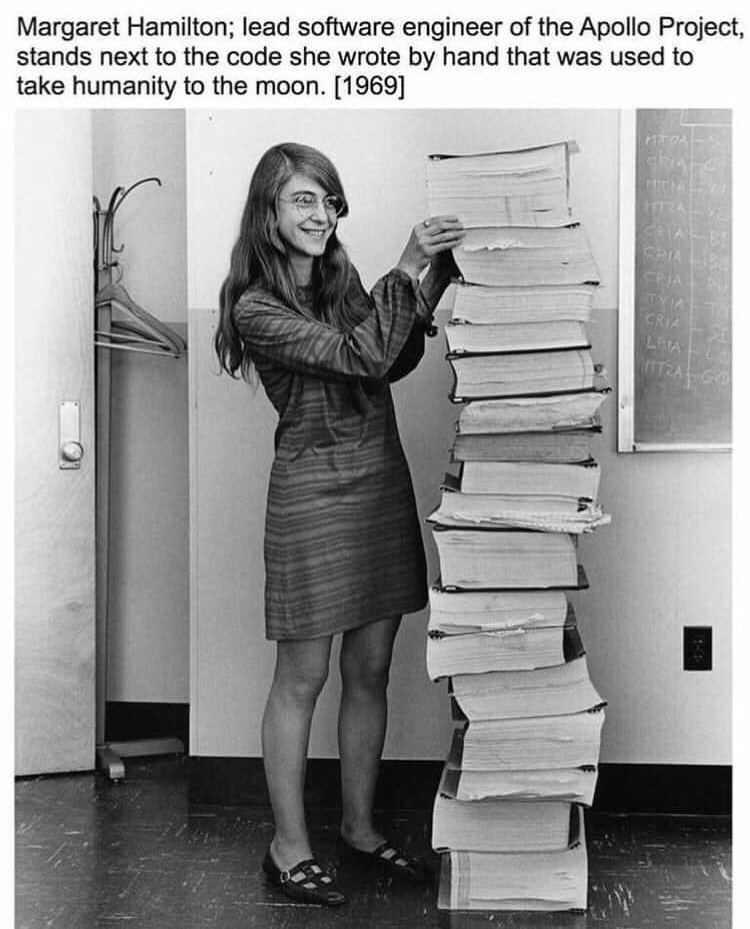
\includegraphics[height=150pt]{margaret_hamilton.jpeg}
\end{figure}
\begin{itemize}
  \item Énorme volume utilisé pour stocker les codes à cette époque, mais très faible puissance de calcul : le module lunaire Appolo 11 était moins puissant qu'une de vos calculettes de lycée !
  \item A mettre en parallèle avec la prochaine ``petite histoire'' parlant de Katie Bouman.
  % https://www.lemonde.fr/sciences/article/2019/04/12/katie-bouman-la-traqueuse-de-trou-noir-propulsee-malgre-elle-superstar-des-femmes-de-science_5449542_1650684.html
\end{itemize}
}
}

\end{document}
